\documentclass[draft,10pt]{article}
\usepackage[utf8]{inputenc}
\usepackage{fixltx2e}
\usepackage{graphicx}
\usepackage{longtable}
\usepackage{booktabs}
\usepackage{amssymb}
\usepackage{hyperref}
\usepackage{mathpazo}
\usepackage{fullpage}
\usepackage{setspace}
\usepackage{amsmath, amssymb, amscd}
\usepackage{algorithm}
\usepackage{algorithmicx}
\usepackage{algpseudocode}
\DeclareMathOperator*{\argmax}{arg\,max}
\title{Spam}
\author{Jon-Michael Deldin}
\date{December 2012}
\begin{document}

\doublespace
\section{Introduction}
Spam is a significant problem in online communities. Spammers advertise their
products, services, viruses, and more to members of these social networks.
Social networks are targeted because they are generally free, and the spammers
can advertise to users via direct messaging or indirect communication (e.g.,
comments on a post). This severely degrades the legitimate user's experience,
affects the website's search engine ranking, and tarnishes the website's
public image.

One social network suffering from spam is
AskNature\footnote{\url{http://www.asknature.org} }. AskNature is a free,
online database of biomimetic~\cite{benyus} solutions. Members can create a
profile, comment on articles, create and read articles, and participate in
forums. Unfortunately, spammers take advantage of the open user registration
and inundate the site with illegitimate accounts, such as the one shown in
Fig.~\ref{fig:spam-profile}. Since the site opened in November 2008, the staff
detected nearly 20,000 spam profiles, in contrast to almost 9,000 legitimate
profiles\footnote{As of November 28, 2012 }. The site has coped with a few
heuristics tools that check for links and HTML, but they are run only to
detect profiles -- a human still inspects and bans users.

\begin{figure}[b]
  \centering
  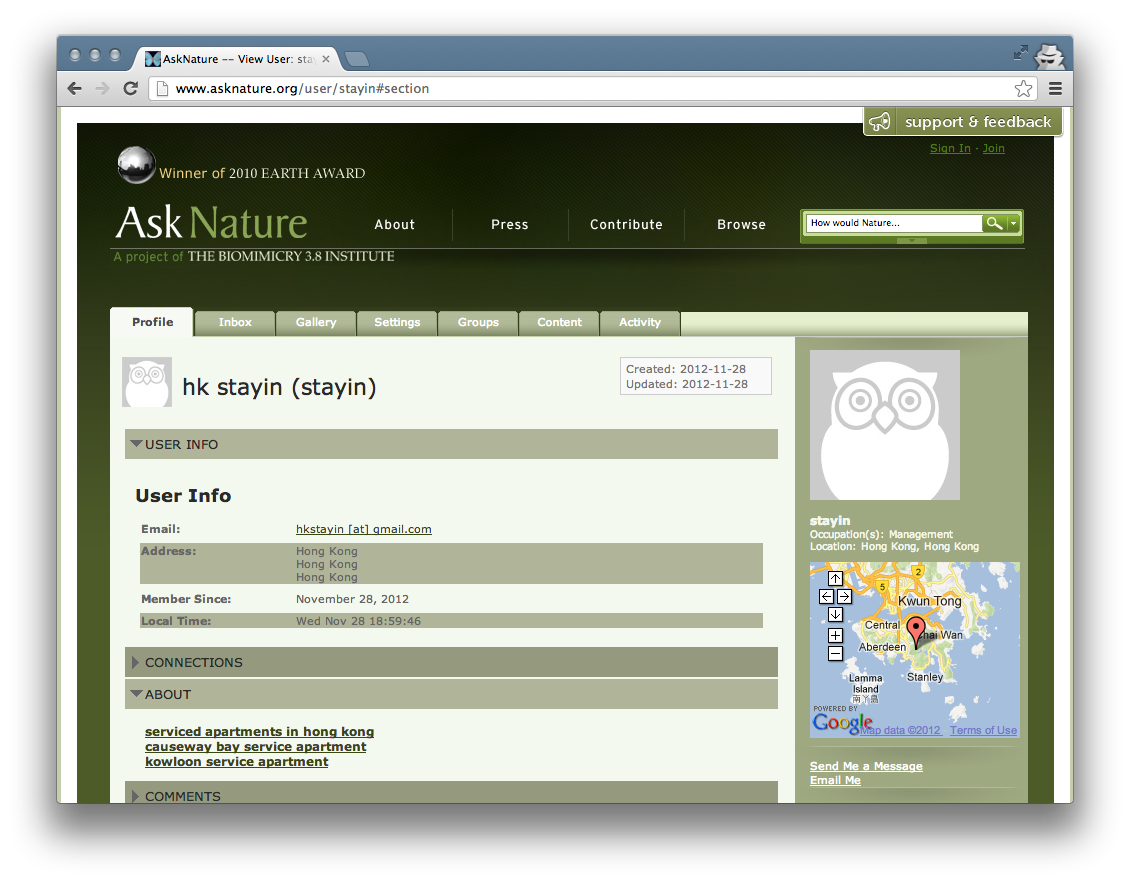
\includegraphics[width=\textwidth]{fig/spam-profile.png}
  \caption{This screenshot of a spam profile shows the "about" text the spammer
    enters, along with the first name ("hk"), last name ("stayin"), username
    ("staying"), and the spammer's address.}
  \label{fig:spam-profile}
\end{figure}

% FIXME: Check again
In this project, I developed a naive Bayes classifier for detecting spam
profiles based on the user's biography\footnote{I will be using ``biography''
  and ``profile'' interchangeably.}. The goal is to determine whether
an account is spam or ham (i.e., a legitimate account) based on the plain text
of the profile. I hypothesized a unigram bag of words model where each word is
represented phonetically is more accurate than representing the words as
themselves. Matching words based on their pronunciation should capture some
misspellings, narrowing the search space of the classifier.

To test this, I performed the following experiments:

\begin{enumerate}
\item Determine the ratio of spam to ham yielding the highest accuracy
\item Determine the minimum number of characters for a biography yielding
  the highest accuracy
\item Determine which n-gram model yields better results for both word and
  character grams
\item Determine whether smoothing probabilities improves accuracy in word-gram
  models
\end{enumerate}

\section{Naive Bayes Classifier}
The research presented here utilizes a naive Bayes classifier to classify spam
and ham biographies. These classifiers are very effective for classifying
documents~\cite[p182]{mitchell}, and they are widely used in email spam
filters~\cite{which-nb}. This classifier uses the maximum a posteriori
estimate to predict which class a document belongs to. The ``naive''
assumption is that each attribute is independent of another, which simplifies
computing a predicted class $v$ to
\[ v = \argmax_{x\in X}\ \Pr(x)\prod_i{\Pr(a_i|x)}, \]
where $X$ is the set of possible classes (e.g., spam and ham), and $a_i$ is an
attribute (i.e., a term). The probability of an attribute given a class is
often computed as a maximum likelihood estimate ({\sc mle}):
\[ \Pr(a_i|x) = \frac{{\textsc{count}_x}(a_i)}{N_x}, \] where
$\textsc{count}_x$ returns the number of occurrences of $a_i$ in the vector of
attributes $<a_1, a_2, \ldots, a_d>$ belonging to class $x$, and $N_x$ is the total number of attributes
for class $x$~\cite[p177]{mitchell}.

{\sc mle} is not without its faults. When the number of times an event occurs
is small, the probability will be zero, which will overfit the data.
Fortunately, additive smoothing (Laplace smoothing) combats this by adding a
smoothing parameter $\alpha$:
\[ \Pr(a_i|x) = \frac{{\textsc{count}}_x + \alpha}{N_x + \alpha d} \]
% TODO: Find a replacement citation for ai-class.com

In text classification, a bag-of-words model is typically used to capture the
frequency of each term appearing in a document. The attributes/terms are words
or characters broken up into $n$-grams, where a unigram corresponds to a
single word (e.g., bag = \{``not'', ``secret''\}), a bigram corresponds to two
words (e.g., bag = \{``not-secret''\}), etc.

\section{Evaluation}
$k$-fold cross-validation, described in Algorithm~\ref{algo:crossvalidation},
is used to compare the performance of the classifier with different models.
Cross-validation will return a confusion matrix -- a table of false positives
(ham marked as spam), false negatives (spam marked as ham), true positives
(spam), and true negatives (ham)\footnote{For brevity, $fp$ will denote a
  false positive, $tn$ will denote a true negative, and so on.}. This
matrix results in the metrics summarized in Table~\ref{table:metrics}. In
this paper, high accuracy is important because it will classify more spam and
ham, but it should not come at the cost of low precision (i.e., more
legitimate users marked as spammers).

\begin{table}[t]
  \centering
  \caption{Summary of evaluation metrics~\cite{eval}. Fewer false positives
    are represented by a higher precision, and fewer false negatives are
    represented by a higher recall rate.}
  \label{table:metrics}
  \begin{tabular}{lcl}
    \toprule
    metric & formula & measures \\ \midrule
  accuracy & $\frac{tp + tn}{tp + fp + fn + tn}$ & correctly predicted classes \\
  precision & $\frac{tp}{tp + fp}$ & correctly predicted positive classes\\
  recall & $\frac{tp}{tp + fn}$ & how sensitive the classifier is to input \\\bottomrule
  \end{tabular}
\end{table}

\begin{algorithm}[b]
  \caption{$k$-fold cross-validation described by~\cite[p147]{mitchell}}
  \begin{algorithmic}
    \Function{CrossValidate}{data, $k$}
    \State partitions $\gets$ divide data into $k$ disjoint subsets
    \For{$i \gets 1 \to k$}
    \State{$T \gets$ data $\setminus\ \mathrm{partitions}_i$}
    \State{{\sc train}($T$)}
    \State{{\sc classify}($\mathrm{partitions}_i$)}
    \State \Return{confusion matrix}
    \EndFor
    \EndFunction
  \end{algorithmic}\label{algo:crossvalidation}
\end{algorithm}

\section{Corpus}
The data consist of user biographies -- Unicode text fields -- spanning
2008-09-03--2012-11-28. These profiles\footnote{``Profile'' and ``biography''
  will be used interchangeably from this point forward.} are from AskNature's
MySQL database, and the spam ones were manually annotated by AskNature staff
during that period. Procuring the corpus involves the following steps:

\begin{enumerate}
\item Select non-empty biographies from all active and banned (spam) users
\item Sanitize each biography according to Algorithm~\ref{algo:preprocess}
\item Save each biography to disk as plain text for easier distribution
\item Determine the mean biography length
\item Segment the samples into training and testing sets according to
  Algorithm~\ref{algo:segment}
\end{enumerate}

\subsection{Mean Biography Length}
In order to maximize the performance of a classifier, appropriate documents
must be selected. Empty samples are obviously not useful in classifying
profiles, and samples with one or two words are unlikely to add reliable
information. One way to determine a minimum count is to take the mean word
counts across spam and ham samples. As shown in
Table~\ref{table:corpus-stats}, the data include more spam accounts than ham,
and those spam accounts have fewer words per biography on average. The wide
standard deviation for both classes is explained by two factors: Users are not
required to fill out the biography field, and even if they choose to, no
stated length requirements exist. These results indicate the floor of the
minimum mean should be used avoid rejecting too much data. Applying a minimum
length of 32 words per biography reduces the samples down to 4,725 spam
entries and 1,730 ham entries.

\begin{table}[t]
  \centering
  \caption{Summary statistics for the non-empty biographies processed
    according to Algorithm~\ref{algo:preprocess}.}
  \label{table:corpus-stats}
  \begin{tabular}{lccc}
    \toprule
    Class & $N$ & Mean Length (words) & $\sigma$\\ \midrule
    Spam  & 18,588 & 32.6 & 92.4 \\
    Ham   & 3,287  & 63.7 & 104.6 \\
    \bottomrule
  \end{tabular}
\end{table}

\begin{algorithm}[b]
  \begin{enumerate}
  \item Sanitize all HTML by retaining just the \texttt{innerHTML} (the
    content between start and closing tags). For example, \texttt{<a
      href="http://example.com">link</a>} becomes \texttt{link}.
  \item Remove all URLs
  \item Replace excess whitespace with single spaces
  \end{enumerate}
  \caption{Preprocessing routine for biographies}
  \label{algo:preprocess}
\end{algorithm}

\begin{algorithm}[t]
  \caption{Segmenting the data samples into training and test sets}
  \label{algo:segment}
  \begin{enumerate}
  \item Create a list of all profiles and randomize it
  \item Select all entries with biographies of 32 or more words
  \item For each class (ham and spam), randomly select 100 entries for testing
    and write to a new \texttt{pruned/testing} directory.
  \item Write the remaining samples to \texttt{pruned/training}
  \end{enumerate}
\end{algorithm}


\section{Methods}

In this section, I describe the methods used to determine an optimal naive
Bayes classifier for classifying spam user profiles on AskNature.

\subsection{Determining the ratio of spam to ham}
An important first step is determining what ratio of spam
To evaluate what ratio of spam to ham would yield a stronger classifier, the
following test was performed.

\begin{algorithm}[b]
  \caption{Determine the ratio of spam:ham messages with the greatest accuracy.}
  \begin{algorithmic}
    \Function{FindBestRatio}{samples, $n$}
    \Comment{Takes a set of $n$ samples}
    \State spam $\gets$ {\sc shuffle}(samples $\setminus $ ham)
    \Comment{Randomizes the order of samples}
    \State ham $\gets$ {\sc shuffle}(samples $\setminus $ spam)
    \State best-accuracy $\gets 0$
    \State best-ratio $\gets \emptyset$
    \\

    \For{$i \gets 0.0 \to 1.0$, step $\gets 0.01$}
    \State ham-ratio $\gets ni$
    \State spam-ratio $\gets n(1 - i)$
    \State limited-samples $\gets$ {\sc take}(ham, ham-ratio) $\cup$ {\sc take}(spam, spam-ratio)
    \\

    \State {\sc cross-validate}(limited-samples)

    \If{accuracy $>$ best-accuracy}
    \State{best-accuracy $\gets$ accuracy}
    \State{best-ratio $\gets$ \{ham-ratio, spam-ratio\}}
    \EndIf
    \EndFor
    \State \Return{best-ratio, best-accuracy}
    \EndFunction
  \end{algorithmic}\label{algo}
\end{algorithm}
\subsubsection{Table of results}
\label{sec-2-2-1}

5 iterations of 3000 cap. Mean and standard devs.
\begin{tabular}{lllllllllllllll}
\end{tabular}
\subsubsection{Selection}
\label{sec-2-2-2}
\subsubsection{Preprocessing}
\label{sec-2-2-3}
\subsubsection{Determining the Minimum Number of Characters}
\label{sec-2-2-4}

We needed to prune. We ran a Naive Bayes Classifier with both unigram and
bigram word models to determine that 18 character sized bodies would give the
greatest accuracy (94.86\% accuracy on 1,000 sample, k=100 cross validation)
\subsection{Naïve Bayes Classifier}
\label{sec-2-3}
\subsubsection{Bag of Words}
\label{sec-2-3-1}
\subsubsection{Bag of Phonetics}
\label{sec-2-3-2}
\subsection{Implementation}
\label{sec-2-4}
\section{Results}
\label{sec-3}
\subsection{F-score}
\label{sec-3-1}

STASTICAL SIGNIFICANCE OF ACCURACY DIFFERENCE
\section{Discussion}
\label{sec-4}
\section{Conclusion}
It would be good to combine this with another one -- to form an ensemble (ref
9,22 from spam paper)
\label{sec-5}



\bibliographystyle{plain}
\bibliography{refs}

\end{document}
